\documentclass{beamer}
\usepackage[utf8]{inputenc}
\usepackage[T1]{fontenc}
\usepackage[french]{babel}

\usepackage{amsmath}
\usepackage{amssymb}
\usepackage{color}
\usepackage{graphicx}
\usepackage[normalem]{ulem}

\usetheme{CambridgeUS}
\title[Projet de SGBD]{Jeux vidéos}
\author[ENSEIRB-MATMECA]{Yvon Garbage, Pierre Lefebvre, Grégoire Pichon}
\institute[S7]{ENSEIRB-MATMECA}
\date{\today}
%\date{}

\setbeamercolor{title}{bg=red!65!black,fg=white}

\begin{document}

\setlength{\unitlength}{1cm}

\begin{frame}{Présentation}

\titlepage

\end{frame}

\section*{Introduction}
\begin{frame}
\begin{block}{Sujet}
Gérer une \textbf{communauté de joueurs} de jeux vidéos. Les joueurs doivent pouvoir \textbf{commenter et juger des commentaires} sur différents jeux. Chaque jeu est lié à \textbf{différentes catégories et plateformes}.

\end{block}

\begin{block}{Objectifs}
\begin{center}
\begin{itemize}
  \item{modélisation du problème,}
  \item{réalisation de requêtes en SQL,}
  \item{gestion de la cohérence de la base,}
  \item{développement d'une interface aux requêtes.}
\end{itemize}
\end{center}
\end{block}
\end{frame}

\section{Modélisation}
\subsection{Précisions quant au sujet}
\begin{frame}
\begin{block}{Choix effectués}
\begin{center}
\begin{itemize}
\item un joueur doit avoir une catégorie et une plateforme préférées,
\item un joueur ne peut noter un jeu qu'une fois,
\item un joueur ne peut critiquer un commentaire qu'une fois,
\item un joueur ne peut pas critiquer un commentaire qu'il a émis,
\item les dates sont cohérentes.
\end{itemize}
\end{center}
\end{block}
\end{frame}

\subsection{Modèle conceptuel}
\begin{frame}
\begin{center}
\begin{figure}[t]
  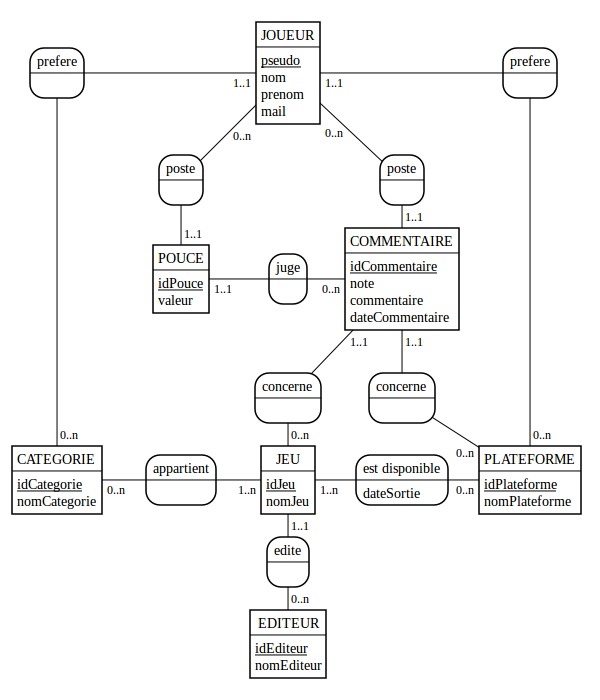
\includegraphics[scale=0.36]{modele_conceptuel.png}
\end{figure}
\end{center}
\end{frame}

\subsection{Modèle relationnel}
\begin{frame}
\begin{block}{Modèle relationnel}
\begin{center}
\begin{figure}[t]
  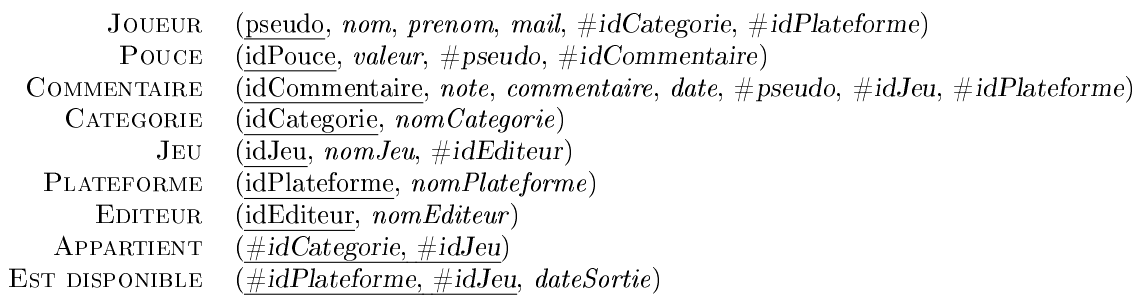
\includegraphics[scale=0.3]{modeleR.png}
\end{figure}
\end{center}
\end{block}
\end{frame}

\section{Requêtes}
\subsection{Classement des jeux}
\begin{frame}
\begin{block}{Requête de classement des jeux}
\begin{center}
\begin{figure}[t]
  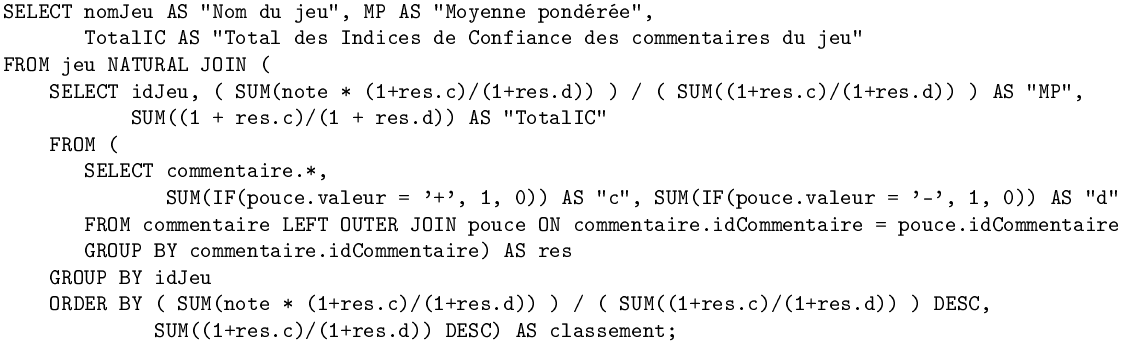
\includegraphics[scale=0.3]{requete.png}
\end{figure}
\end{center}
\end{block}
\end{frame}


\section{Cohérence de la base}
\subsection{Gestion de la cohérence}
\begin{frame}
\begin{block}{Gestion de la cohérence}
\begin{itemize}
  \item {\textbf{Clés étrangères} \\
      \footnotesize{Ex:~~\texttt{ALTER TABLE jeu ADD CONSTRAINT fk1\_jeu FOREIGN KEY (idEditeur) REFERENCES editeur (idEditeur);}}}

  \item {\textbf{Actions en cascade} \\
    \footnotesize{Ex:~~\texttt{ALTER TABLE estDisponible ADD CONSTRAINT fk1\_estDisponible FOREIGN KEY (idJeu) REFERENCES jeu (idJeu) \textbf{ON DELETE CASCADE;}}}}
  \item{  \textbf{Contrainte \texttt{UNIQUE} sur certains attributs}\\
    \footnotesize{Ex:~~\texttt{nomPlateforme VARCHAR(128) UNIQUE}}}
  \item {\textbf{Contrôles réalisés en PHP}\\
    \footnotesize{Ex: un joueur ne peut apprécier ses propres commentaires}}

\end{itemize}
\end{block}
\end{frame}

\section{Interface}
\subsection{Description de l'interface}
\begin{frame}
\begin{block}{Interface}
\begin{center}
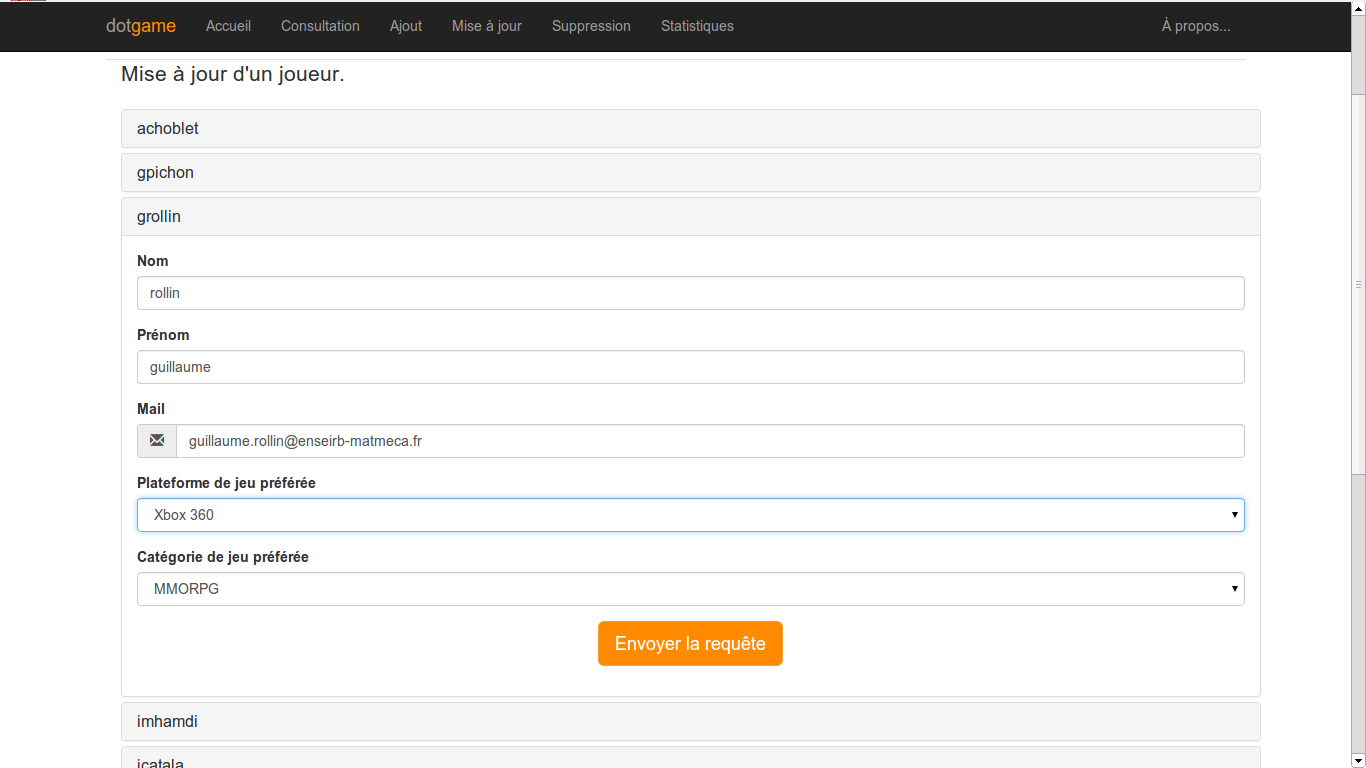
\includegraphics[scale=0.20]{capture2.png}
\end{center}
\begin{itemize}
\item Site web
\item PHP/MySQL
\item Bootstrap / jQuery
\end{itemize}
\end{block}
\end{frame}

\section*{Conclusion}
\begin{frame}
\begin{block}{Conclusion}
\begin{itemize}

\item{difficulté du choix des contraintes,}
\item{optimisations supplémentaires possibles,}
%\item{le vrai cas d'étude: la prise en compte des cas d'utilisation,}

\item{toutes les requêtes ont été réalisées,}
\item{base cohérente,}
\item{interface simple et claire.}

\end{itemize}
\end{block}
\end{frame}


\section{Conclusion}
\subsection{Remerciements}
\begin{frame}
  \begin{center}
    \large{Merci de votre attention.}
  \end{center}
  \end{frame}


\end{document}
